\documentclass[xcolor=dvipsnames]{beamer}

\usetheme{Frankfurt}

\usenavigationsymbolstemplate{}

\usepackage{amsmath}
\usepackage{amsfonts}
\usepackage{amssymb}
%\usepackage{xcolor}
\usepackage{movie15}
\usepackage{graphicx}
\usepackage{hyperref}
\usepackage{ulem}
\usepackage{cancel}
\usepackage{marvosym}
\usepackage{framed}
\usepackage{epstopdf}
%\definecolor{black}{RGB}{0,255,0}
%\definecolor{white}{RGB}{255,242,0}
%\usecolortheme[RGB={255,174,201}]{structure}

\usecolortheme[RGB={0,0,96}]{structure}

\usepackage[labelformat=simple]{subfig}

\renewcommand{\thesubfigure}{\relax}

\newcommand{\vs}{\vspace{7mm}}
\newcommand{\diff}[2]{\dfrac{\textnormal{d} #1}{\textnormal{d} #2}}
\newcommand{\specialcell}[2][c] { \begin{tabular}[#1]{@{}c@{}}#2 \end{tabular}}
\newcommand{\pderiv}[2]{\frac{ \partial #1}{\partial #2}}

\newcommand{\be}{\begin{enumerate}}
\newcommand{\bec}{\begin{enumerate} \item[]} %For chained enumerations without content, to cut directly to letters easily.
\newcommand{\ee}{\end{enumerate}}
\newcommand{\bi}{\begin{itemize}}
\newcommand{\ei}{\end{itemize}}

\newcommand{\slide}[2][]{\begin{frame}\frametitle{#1}#2\end{frame}}
\newcommand{\mat}[1]{\left [ \begin{array}{ccc} #1 \end{array} \right ]}


\title[Tsunami Modeling]{Tsunami Modeling in Parabolic Bays}
\author{Matthew Harris \\ John Pender}
\date{\today}
\institute{University of Alaska Fairbanks}

%% Version 0.1

\begin{document}
	\begin{frame}
		\titlepage
		{\inserttotalframenumber}
	\end{frame}
	
	\slide[Outline]{\tableofcontents}
	
%	% 1  Introduction
\section{Introduction}

% 1.1  Define tsunami wave (versus wind wave)
	\slide[Tsunami Waves] {
	\begin{enumerate}
		\item Tsunami waves are long waves, $\lambda>> D$ or $\frac{D}{\lambda}\approx0$.
		
		\item Wind waves are short waves, $\lambda\not>\not> D$ or $\frac{D}{\lambda}\not\approx 0$.
		\end{enumerate}
		\centering
		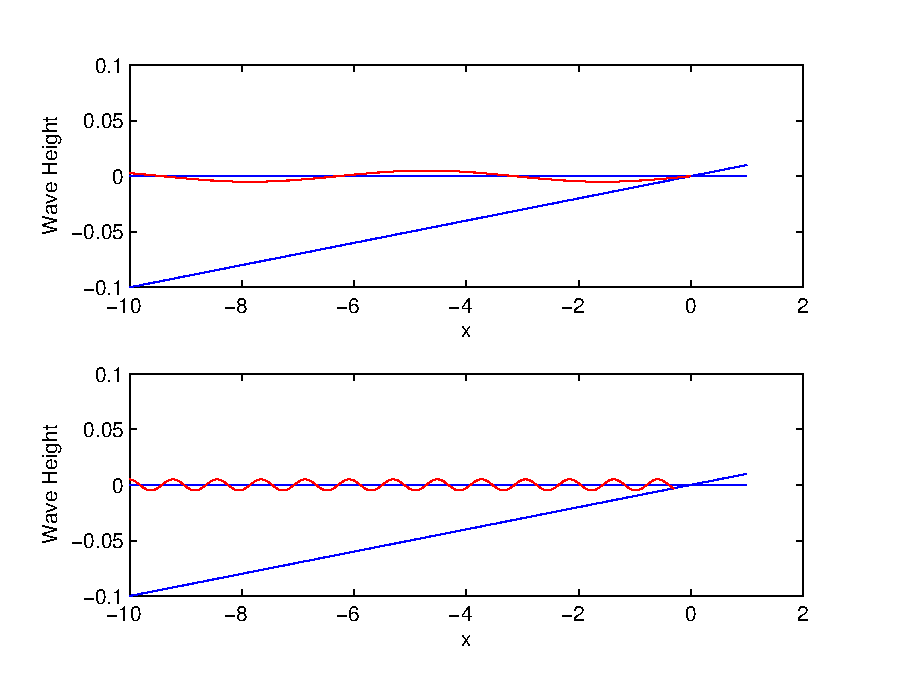
\includegraphics[width=.8\textwidth]{bay/wave_comp.eps}
	}
% 1.1.1  Typical causes of tsunami waves
	\slide[Causes of Tsunami Waves] {
	\begin{tabular}{|l|l|}\hline
		Rock Slides--Chehalis Lake&Earthquakes\\
			 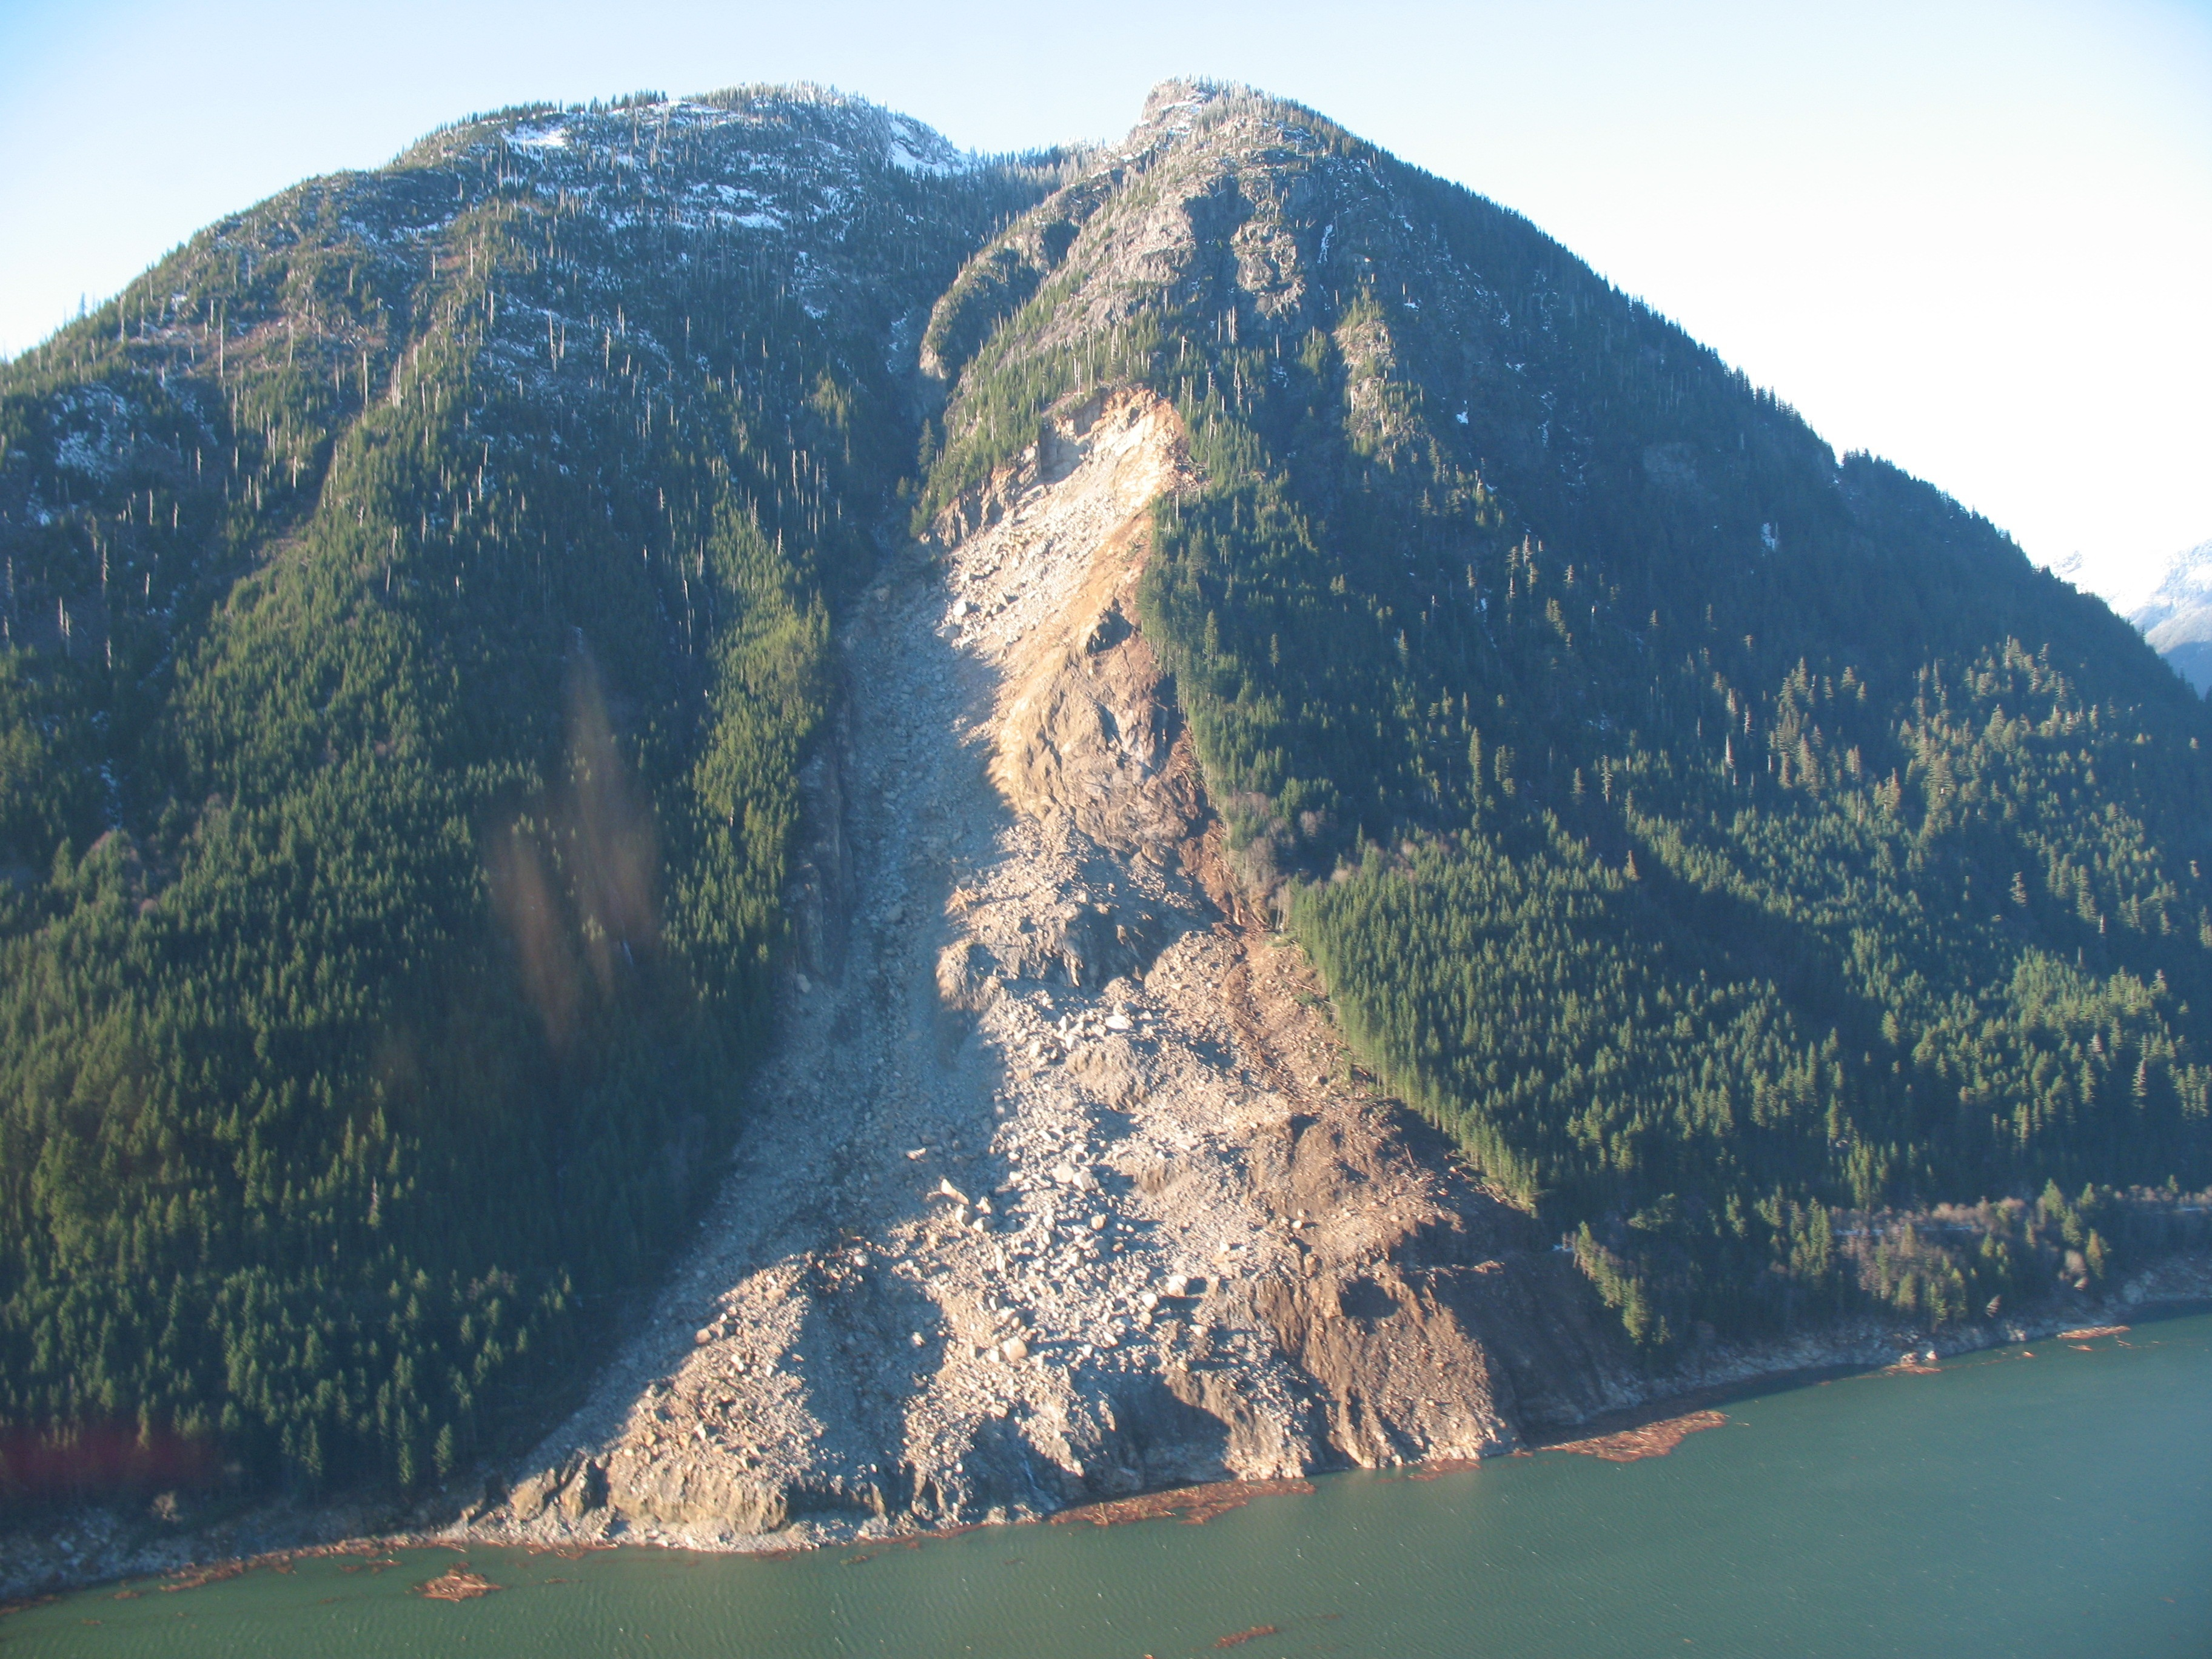
\includegraphics[width=.4\textwidth]{causes/Landslide.jpg}%http://wikimapia.org/22797805/Chehalis-Lake-Rock-Slide
			&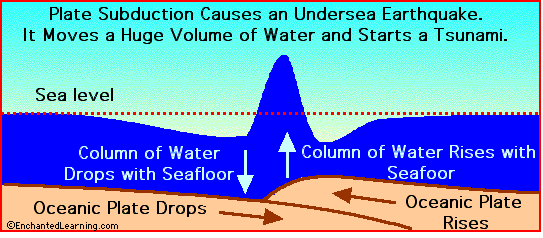
\includegraphics[width=.5\textwidth]{causes/Earrthquake.png}\\\hline%http://www.enchantedlearning.com/subjects/tsunami/\\\hline
			Asteroid Impact&Glacier Calving\\
			 ~ ~ 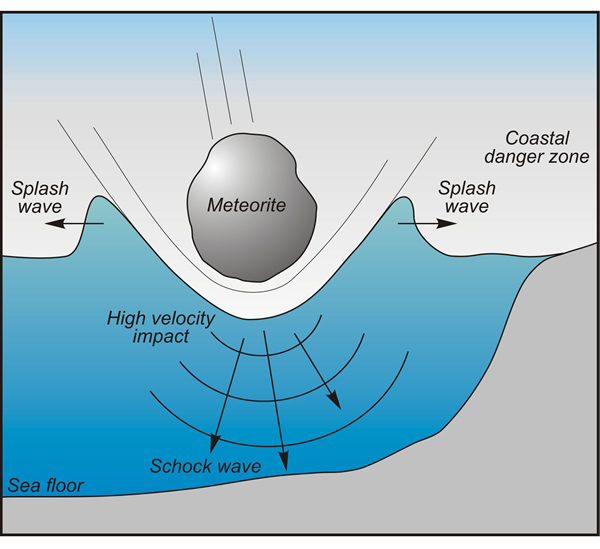
\includegraphics[width=.3\textwidth]{causes/Asteroid.jpg}%http://mail.colonial.net/~hkaiter/asteroidbelt.html
			&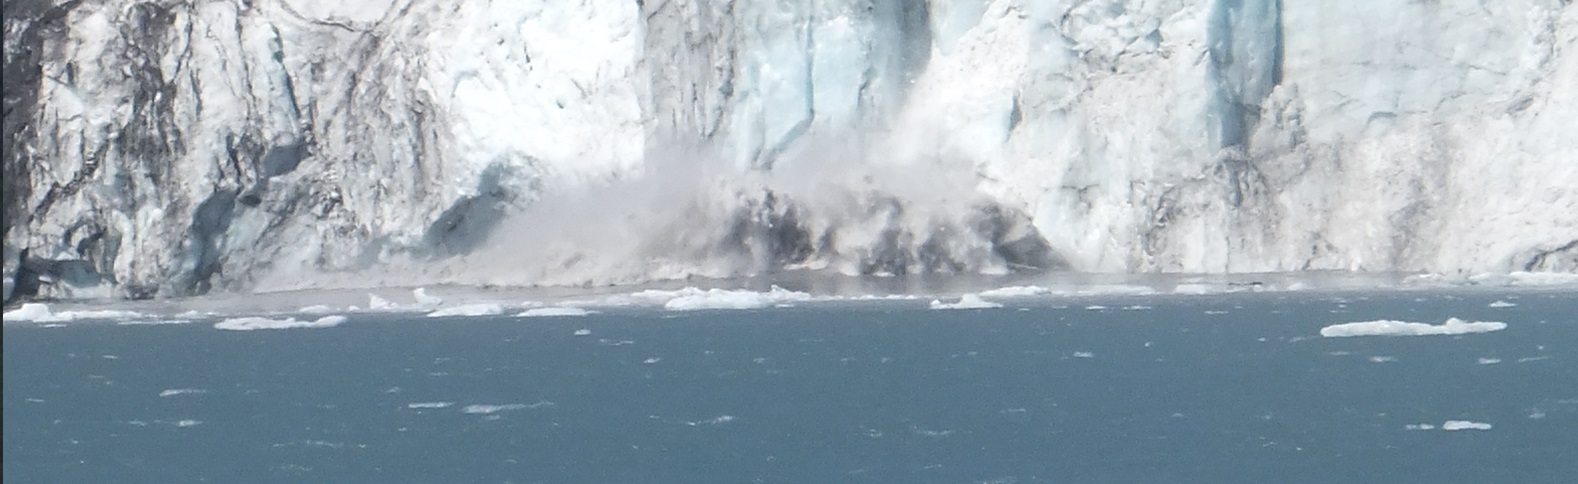
\includegraphics[width=.5\textwidth]{causes/Calving.jpg}\\\hline
	\end{tabular}
	}


\slide[Purpose of Research]{
\bi	\item Faster numerical modeling of wave run-up
	\bi	\item Closed bays with a steep wall
		\item Carrier-Greenspan transformation generalized by Rybkin-Pelinovsky-Didenkulova.
		\item $<1$ min vs. 2 days computation time
	\ei
\ei
}
% 1.1.2  Include pictures/videos ? from trip and elsewhere
% 1.2  Purpose of our research
	\slide[Introduction to the Problem]{
		Mathematical modeling of tsunami run-up
		\bi	\item Numerous real-world applications
			\item Involves solving non-linear partial differential equations
		\ei
		Our REU program focused on
		\bi	\item Bays of U-Shaped bays of finite length.
			\item Spectral method for finding numerical series solutions.
		\ei
	}
	% 2  Previous Work
% 2.1  Problem setup picture(s) (which shows all variables)
% 2.2  Assumptions
% 2.3  NLSWEs ? derived from conservation of mass and Newton?s Second Law under assumptions (Just mention, not actually derive)
% 2.3.1  Mention that the SWEs have no dispersion ? there is very little dispersion near shore so this is where SWEs apply? fact check and/or more info
% 2.4  Very brief overview of how NLSWEs are linearized for arbitrary cross section
% 2.4.1  Properties of new system
% 2.4.2  Include equations to get back to physical variables
% 2.4.3  Analytical F(?) and thus W(?) for |y|^m case

	\begin{frame}
		\frametitle{Introduction to the Bay Shapes}
		In the field of Tsunami run-up research, there are several natural bay shapes to examine:
		\begin{itemize}
			\item The plane beach;
			\item Bays of parabolic cross-section;
		\end{itemize}
		There has been extensive study of the plane beach and bays of parabolic cross-section, but tsunami behavior in bays of general U-shaped bays of finite length has not been examined.
		
		In each case, we assume that the bottom profile is separable: \emph{i.e.}
		\[   z(x,y) = f(y) - h(x)  \]
		where $z(x,y)$ is the bottom profile, $f(y)$ is an arbitrary function and $h(x)$ is an arbitrary non-negative function.
	\end{frame}

	\slide[The Plane Beach]{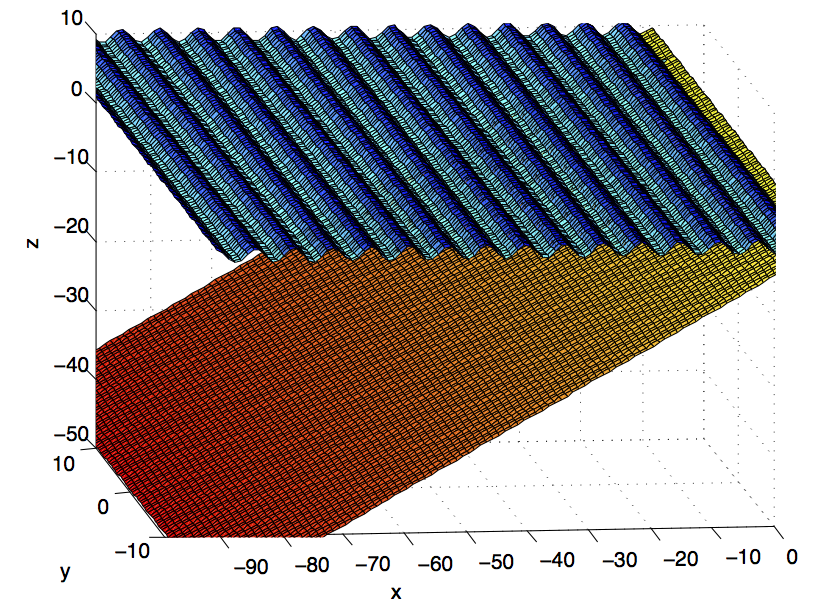
\includegraphics[width=\linewidth]{bay/planebeach.png}}

	\begin{frame}
	\frametitle{The Plane Beach}
		Characteristics of the plane beach:
		\begin{itemize}
			\item Constant slope;
			\item Uniform across y-axis;
			\item Can be simplified to 2 dimensions.
		\end{itemize}
		This is the problem examined in the famous 1958 paper of Carrier and Greenspan. They showed that in this case, explicit solutions to the shallow water wave equations were possible.
	\end{frame}

	\slide[Bays of Parabolic Cross-section]{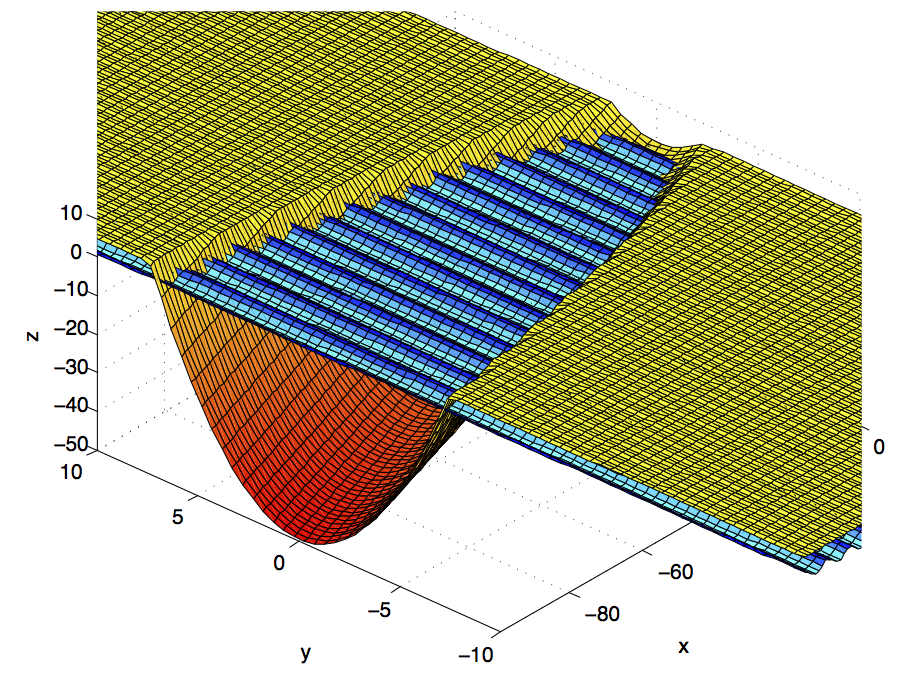
\includegraphics[width=\linewidth]{bay/parabolicbay.png}}

	\begin{frame}
		\frametitle{Bays of Parabolic Cross-section}
		Characteristics of bays of parabolic cross-section:
		Characteristics of bays of parabolic cross-section:
		\begin{itemize}
			\item Constant slope;
			\item Parabolic cross-section along y-axis;
			\item Behavior of waves in such a channel can still be simplified to 2 dimensions.
		\end{itemize}
		This more complicated problem was analyzed in a recent paper by Dr. Ira Didenkulova and Dr. Efim Pelinovsky, in which they showed that it was possible to reduce this problem to one that is analogous to the 2-dimensional case, and thus analytical solutions are possible for the infinite length case.
	\end{frame}

	

	\begin{frame}
		\frametitle{Further Terminology}
		There are a few other terms we use:
		\begin{itemize}
			\item $\eta(x,t)$ is the perturbation away from the normal water level at time $t$ and distance $x$ from shore.
			\item $H(x,t)$ is the total water depth. Note that $H(x,t) = h(x) + \eta(x,t)$.
			\item Note that for all the cases we will consider, $h(x) = -\alpha x$, where $\alpha$ is a non-negative constant. Since $x$ is typically negative in our domain, $h$ will usually be non-negative, and $H$ must always be non-negative.
		\end{itemize}
	\end{frame}

	

	\begin{frame}
		\frametitle{Wave Equation*}
		% Put the basic assumptions and talk about the general idea but do not derive everything
		% It took too much time when I gave my talks and it does not help to gain a better understanding
		% We will need the time to get through the results and explaining how the solution works
		% Ill leve it up to you to talk about eulers eq and the C of Mass eq and the assumptions/ make the slides you want.
		From this point forward, we use the symbol $u$ to represent $\bar{u}$.  Thus,
		\begin{framed} \begin{align}
			\frac{\partial S}{\partial t} + \frac{\partial}{\partial x}(uS) &= 0, \label{swe1}\\
			\frac{\partial u}{\partial t} + u \frac{\partial u}{\partial x} + g \frac{\partial H}{\partial x} &= g \frac{dh}{dx}. \label{swe2}
		\end{align} \end{framed}
		These are the wave equations that we will attempt to solve for our bays.
		% I will mention no dispersion and the compairison when you are done with your part (no slide)
	\end{frame}


\section{Mathematical Setup}

	\begin{frame}
		\frametitle{Transformation to $\sigma$, $\lambda$}
		We begin with the non-linear shallow water equations
		\begin{align} 
			\tag*{\eqref{swe1}}
			\frac{\partial S}{\partial t} + \frac{\partial}{\partial x} (uS) &= 0  \\
			\tag*{\eqref{swe2}}
			\frac{\partial u}{\partial t} + u \frac{\partial u}{\partial x} + g \frac{\partial H}{\partial x} &= g \frac{dh}{dx}
		\end{align}
		where $S$ is the cross-sectional area, $u$ is the averaged flow velocity, and $H = \eta(x,t) + h(x)$, where $h$ is unperturbed water depth and $\eta$ is the height of the perturbation.
		
		We have initial conditions that at $t=0$, $u(x,0) = 0$ and $\eta(x,0) = \eta_0(x)$, and boundary conditions that at $x=L$, $\frac{u(x_L,t)}{F(\sigma_{x_L})}=0$ 'wall' and that at the moving shoreline, $u(x,t)$ is bounded.
		
	\end{frame}


\begin{frame}
\frametitle{Riemann Invariants}
From these two equations, we can find Riemann Invariants
\[
I_\pm = u \pm \int \sqrt{\frac{g}{S}\frac{dS}{dH}} dH + g \alpha t
\]
Applying these to \eqref{swe1} and \eqref{swe2}, we get
\begin{equation}\label{invariants1}
\frac{\partial I_\pm}{\partial t} + c_{\pm} \frac{\partial I_\pm}{\partial x} = 0
\end{equation}
where
\[
c_\pm = u \pm \sqrt{g S \frac{dH}{dS}}.
\]
Note that we can write \eqref{invariants1} as
\[
\frac{\partial (I_\pm, x)}{\partial (t,x)} + c_\pm \frac{\partial(t, I_\pm)}{\partial (t,x)} = 0.
\]
\end{frame}

\begin{frame}
\frametitle{Hodograph Transform}
We apply a hodograph transform with Jacobian $\dfrac{\partial (t,x)}{\partial(I_+, I_-)}$. This Jacobian will be zero if, and only if, the wave breaks before it reaches shore. After applying the transform, we see that
\[
\frac{\partial(I_\pm,x)}{\partial(I_+,I_-)} + c_\pm \frac{\partial (t, I_\pm)}{\partial(I_+,I_-)} = 0,
\]
which can be written as
\begin{equation}\label{hodograph}
\frac{\partial x}{\partial I_\pm} - c_\mp \frac{\partial t}{\partial I_\pm} = 0.
\end{equation}
\end{frame}

\begin{frame}
\frametitle{Change of Variables}
We define two new variables:
\[
\lambda = \frac{I_+ + I_-}{2} \text{ and } \sigma = \frac{I_+ - I_-}{2}.
\]
Notice that this implies that
\begin{equation} \label{siglam}
\lambda = u + \alpha g t \text{ and } \sigma = \int_0^H \sqrt{\frac{g}{S} \frac{dS}{dH}}dH.
\end{equation}
We also define
\[
F(\sigma) = c_+ - c_- = 2 \sqrt{gS \frac{dH}{dS}}.
\]
\end{frame}

\begin{frame}
\frametitle{Change of Variables 2}
In these new variables, \eqref{hodograph} becomes
\[
\frac{\partial^2 t}{\partial \lambda^2} - \frac{\partial^2 t}{\partial \sigma^2} - \left( \frac{2 + \frac{dF}{d\sigma}}{F(\sigma)} \right) \frac{\partial t}{\partial \sigma} = 0,
\]
which, because of how $u,t,$ and $\lambda$ are related in \eqref{siglam}, is equivalent to
\begin{equation}\label{finalu}
\frac{\partial^2 u}{\partial \lambda^2} - \frac{\partial^2 u}{\partial \sigma^2} - \left( \frac{2 + \frac{dF}{d\sigma}}{F(\sigma)} \right) \frac{\partial u}{\partial \sigma} = 0.
\end{equation}
So we can find $t$ and $u$.
\end{frame}

\begin{frame}
\frametitle{Finding a relation for $x$}
In order to find $x$, we also obtain from \eqref{hodograph} that
\[
g \alpha \frac{\partial x}{\partial \sigma} = - u \frac{\partial u}{\partial \sigma} - \frac{F(\sigma)}{2} + \frac{F(\sigma)}{2} \frac{\partial u}{\partial \lambda}.
\]
To integrate this, we define a potential function $\Phi(\sigma,\lambda)$ by
\[
u = \frac{1}{F(\sigma)} \frac{\partial \Phi}{\partial \sigma}.
\]
Then we see that
\[
2 g \alpha x = \frac{\partial \Phi}{\partial \lambda} - \int_0^\sigma F(\sigma) d\sigma - u^2 = \frac{\partial \Phi}{\partial \lambda} - 2gH - u^2.
\]
Hence
\[
\eta = H - h = H + \alpha x = \frac{1}{2g} \left(\frac{\partial \Phi}{\partial \lambda} - u^2 \right)
\]
\end{frame}








\begin{frame}
\frametitle{Backsubstituting to Physical Variables}
We have the following backsubstitution equations:
\[
u = \frac{\phi_\sigma}{F(\sigma)} \text{ and } \eta = \frac{1}{2g}\left(\phi_\lambda - u^2\right)
\]
\[
x = \frac{1}{2g\alpha} \left(\phi_\lambda - 2gH - u^2 \right) \text{ and } t = \frac{\lambda - u}{\alpha g}.
\]
We know that this backsubstitution is possible because the 4-part Jacobian matrix
\[
\frac{\partial (x,t,u,\eta)}{\partial (\sigma,\lambda,\phi_\sigma,\phi_\lambda)}
\]
has a non-zero determinant.
\end{frame}


\begin{frame}
\frametitle{Writing an Equation in Terms of $\Phi$}
We substitute our definition of $\Phi$ into \eqref{finalu} to obtain
\begin{equation}\label{Phieq}
\frac{\partial^2 \Phi}{\partial \lambda^2} - \frac{\partial^2 \Phi}{\partial \sigma^2} - W(\sigma) \frac{\partial \Phi}{\partial \sigma} = 0,
\end{equation}
where
\[
W(\sigma) = \frac{2 + \frac{dF}{d\sigma}}{F(\sigma)}.
\]
We can think of $\sigma$ as a space-like variable and $\lambda$ as a time-like variable. So we have initial conditions at $\lambda = 0$,
\end{frame}


\begin{frame}
\frametitle{Finding $F$ and $W$ for U-shaped bays}
We need to find $F(\sigma)$ for the case of a U-shaped bay ($|y^m|$). Recalling that
\[
F(\sigma)= 2 \sqrt{gS \frac{dH}{dS}} \text{ and } \sigma = \int_0^H \sqrt{\frac{g}{S} \frac{dS}{dH}}dH.
\]
By integrating we can write $S(H)=2\frac{m}{m+1}H^{\frac{m+1}{m}}$ and also
\[
F(H)=2\sqrt{g} \sqrt{\frac{m}{m+1}} \sqrt{H} \text{ and } \sigma=2\sqrt{\frac{g(m+1)}{m}} H^{\frac12}
\]
So
\[F(\sigma)=\frac{m}{(m+1)\sigma}
\]
and
\[
W(\sigma) = \frac{2 + \frac{dF}{d\sigma}}{F(\sigma)}=\frac{m+2}{m\sigma}.
\]

\end{frame}





%	% 3  Our work
\section{2013 REU}

% 3.1  Discuss our specific problem which allows us to apply spectral methods
% 3.1.1  Boundary condition: shore condition and ?wall? at some distance L
% 3.1.1.1  This is a potential problem we must keep track of? eta must be close to zero to avoid significant error.
% 3.1.2  Mention physical examples where ?wall? could exist
% 3.1.2.1  Actual physical wall-like object: dam, glacier, cliff, steep mountain, anything steep enough that does not move can be approximated as a wall
% 3.1.2.2  Point that the wave passes through but does not alter height (analogous to point in the middle of 2 standing waves)
%- 3.2  Go through spectral method for arbitrary m with Bessel solution.
% 3.3  Mention for m=2 this solution is simplified to sin solution
% 3.3.1  Still not fully analytic though because eigenvalues can only be found numerically


%3.11
\begin{frame}
\frametitle{Finding IC's in Terms of $\Phi$}
Old IC's were $u(x,0) = 0$ and $\eta(x,0) = \eta_0(x)$
As
\[
u = \frac{1}{F(\sigma)} \frac{\partial \Phi}{\partial \sigma}.
\]
and
\[
\eta =  \frac{1}{2g} \left(\frac{\partial \Phi}{\partial \lambda} - u^2 \right)
\]
We can write new IC's as
\[
\Phi(\sigma,0) = \int\limits_0^\sigma u_0(x_{\sigma'})F(\sigma')d\sigma'=0 \text{ and } \frac{\partial \Phi(\sigma,0)}{\partial \lambda} = 2g\eta_0.
\]
\end{frame}


\begin{frame}
\frametitle{Finding BC's in Terms of $\Phi$*}
Old BC's were $x=L$, $\frac{u(x_L,t)}{F(\sigma_{x_L})}=0$ 'wall' and that at the moving shoreline, $u(x,t)$ is bounded. As 
\[
u = \frac{1}{F(\sigma)} \frac{\partial \Phi}{\partial \sigma}.
\]
Our new BC's are
\[
\frac{\partial \Phi(\sigma_{x_L},\lambda)}{\partial \sigma} = 0 \text{ and } \frac{\partial \Phi(0,\lambda)}{\partial \sigma} = 0.
\]
\end{frame}


\slide[Boundary Conditions*]{
% I think it is better to start in physical space as we are setting the wall there
% then to find the simga_l for the x_l and to fix that sigma_l
We chose to let:
\begin{align*}
\Phi_\sigma (0,\lambda)=0& ~ ~ ~ ~ \Phi_\sigma (L,\lambda)=0
\end{align*}
As $u(x,t)= \frac{1}{F(\sigma)} \Phi_\sigma(\sigma,\lambda)$
\[
u(x_{\sigma=0},t)=A(t) ~ ~ ~ \text{reflecting wall If wave does not break}
\]
and
\[
u(x_{\sigma_L},t)=0 ~ ~ ~ \text{Reflecting vertical wall}
\]
}




% 3.1.1.1
\slide[Boundary Conditions for a Closed Bay]{
	Neither end of the bay moves
	\[
		\Phi_\sigma (0,\lambda)=0 \qquad \Phi_\sigma (L,\lambda)=0
	\]
	Because $u(x,t)= \frac{1}{F(\sigma)} \Phi_\sigma(\sigma,\lambda)$
	\[
		u(x_{\sigma=0},t)=A(t) ~ ~ ~ \text{reflecting wall If wave does not break}
	\]
	and a reflective vertical wall
	\[
		u(x_{\sigma_L},t)=0
	\]
}
% 3.1.1.1  This is a potential problem we must keep track of? eta must be close to zero to avoid significant error.
\slide[Potential Issue with BC's]{
	We assume that $x_{\sigma_L}=const$ but
	
	\[
	x({\sigma_L},\lambda)=\frac{1}{2g\alpha}\left(  \Phi_\lambda(\sigma_L,\lambda)-2g H(\sigma_L)-\frac{1}{F(\sigma_L)}\Phi_\sigma(\sigma_L,\lambda)\right)
	\]

}



% 3.1.2  Mention physical examples where ?wall? could exist
% 3.1.2.1  Actual physical wall-like object: dam, glacier, cliff, steep mountain, anything steep enough that does not move can be approximated as a wall
% 3.1.2.2  Point out that the wave passes through but does not alter height (analogous to point in the middle of 2 standing waves)
	\slide[Examples of Closed Bays] {
		\begin{columns}
			\begin{column}{.48 \textwidth}
				\bi	\item Lituya Bay
					\item Dammed reservoir
					\item Glacial dams
					\item Standing waves
				\ei
			\end{column}
			\begin{column}{.48 \textwidth}
				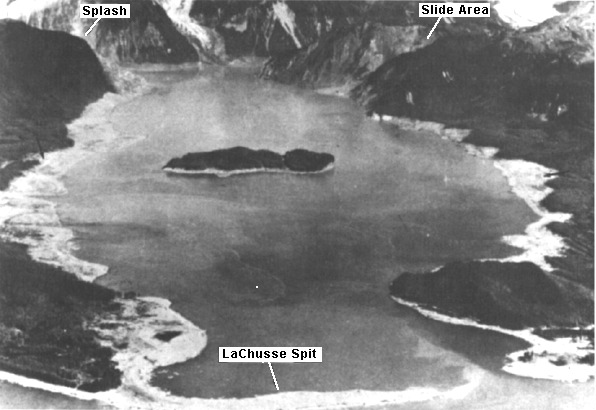
\includegraphics[width=1\textwidth]{bay/lituya.jpg}
			\end{column}
		\end{columns}
	}

	\begin{frame}
		\frametitle{IVBP}
			We wish to solve the following system:
			\begin{tabular}{l l l}
			\text{PDE: }& $\Phi_{\lambda \lambda}$&$=L\Phi$ \\\\
			\text{BC: }& $\Phi_\sigma (0,\lambda)$&$=0$\\
								 & $\Phi_\sigma (L,\lambda)$&$=0$\\\\
			\text{IC: }& $\Phi(\sigma,0)$&=$\int\limits_0^\sigma u_0(\sigma ')F(\sigma ')d \sigma'=0$\\
								 & $\Phi_\lambda(\sigma,0)$&=$2g\eta_0$\\
			\end{tabular}
			$\text{ where }L=\frac{\partial^2}{\partial \sigma^2}+\frac{m+1}{m\sigma}\frac{\partial}{\partial \sigma}$, $\sigma\in [0,\infty]$,and $\lambda\in [0,\infty)$
	\end{frame}
	
	
	
	\begin{frame}
	\frametitle{Solution}
			Assume solutions have the form $\Phi(\sigma,\lambda)=T(\lambda)X(\sigma)$.  We now have
			\begin{align*}
			\Phi_{\lambda \lambda}&=\left(\frac{\partial^2}{\partial \sigma^2}+\frac{m+1}{m\sigma}\frac{\partial}{\partial \sigma}\right)\Phi\\\\
			T''(\lambda)X(\sigma)&=T(\lambda)X''(\sigma)+\frac{m+1}{m\sigma}T(\lambda)X'(\sigma)\\\\
			\frac{T''(\lambda)}{T(\lambda)}&=\frac{X''(\sigma)}{X(\sigma)}+\frac{m+1}{m\sigma}\frac{X'(\sigma)}{X(\sigma)}\\
			\end{align*}
			So $T''(\lambda)=CT(\lambda)$ and $X''(\sigma)+\frac{m+1}{m\sigma}X'(\sigma)=C X(\sigma)$
	\end{frame}
	
	
	\begin{frame}
		\frametitle{Solution 2}
		 We now want to solve the system of ODEs:
		\[X''(\sigma)+\frac{m+1}{m\sigma}X'(\sigma)=C X(\sigma),\]
		\[T''(\lambda)=CT(\lambda)\]
		with conditions
		\[\Phi_\sigma (0,\lambda)=0\text{, }\Phi_\sigma (L,\lambda)=0\]
		\[ \Phi(\sigma,0)=\int\limits_0^\sigma u_0(\sigma ')F(\sigma ')d \sigma'\text{ and }\Phi_\lambda(\sigma,0)=2g\eta_0\]
	\end{frame}



% 3.3  Mention for m=2 this solution is simplified to sin solution
% 3.3.1  Still not fully analytic though because eigenvalues can only be found numerically

	\slide[m=1 case: X] {
		When m=1 (i.e. parabolic bay), we have 
			\[X''(\sigma)+\frac{2}{\sigma}X'(\sigma)=\lambda_n X(\sigma)\]
		which is nicely solved with
			\[ X = A\frac{\sin(\lambda_n \sigma)}{\sigma} + B\frac{\cos(\lambda_n \sigma)}{\sigma} \]
		Using the boundary conditions: $X'(0) = 0$ and $X' (L) = 0$, we find $B=0$ and
			\[ \lambda_n L = \tan(\lambda_n L) \]
		which can be solved implicitly for numerical solutions.
	}
	\slide[m=1 case: $\Phi$] {
			\[ T'' - \lambda_n T = 0 \]
		can be readily solved with
			\[ T = \lambda_n [ A \sin (\lambda_n \lambda) + B \cos ( \lambda_n \lambda) ] \]
		Pulling both X and T together:
			\[ \phi = \lambda_n [ A  \cos (\lambda_n \lambda) - B \sin ( \lambda_n \lambda) ] \frac{\sin (\lambda_n \sigma)}{\sigma} \]
			\[ \psi = \lambda_n [ A  \sin (\lambda_n \lambda) + B \cos ( \lambda_n \lambda) ] \pderiv{}{\sigma} \frac{\sin (\lambda_n \sigma)}{\sigma} \]
		which can, using multiple $\lambda_n$, decompose an initial wave into its components.
			\[ \phi_0 = \sum A \frac{\lambda_n}{\sigma} \sin(\lambda_n \sigma) \qquad \psi_0 = \sum B \frac{1}{\sigma} \sin(\lambda_n \sigma) \]
	}
	
	




%- 3.2  Go through spectral method for arbitrary m with Bessel solution.	
	
	
	
	
	\begin{frame}
	\frametitle{Generalized m}
		 Letting $\alpha=\frac 1m$, $\varphi=X(\sigma)\sigma ^\alpha$, $t=\sigma \sqrt{C}$ and doing some algebraic manipulations we can rewrite 
		\[X''(\sigma)+\frac{m+1}{m\sigma}X'(\sigma)=C X(\sigma)\]
		as
		\[t^2 \varphi_{tt}+t \varphi_t-(\alpha^2+t^2)\varphi=0\]
		Which has well known solutions: the Modified Bessel Functions $I_\alpha(t)$ and $K_\alpha(t)$. Our solutions can be written as $$\varphi=C_1I_\alpha(t)+C_2K_\alpha(t).$$ We can also write our boundary conditions in terms of $\varphi$ as 
		\[\varphi(0)=0\text{ and }-\alpha\varphi(L\sqrt{c})+L\varphi'(L\sqrt{c})=0\]
	\end{frame}
	
	
	\begin{frame}
		\frametitle{Modified Bessel Functions}
		\centering
		\begin{tabular}{|c|c|}\hline
		$I_\alpha(t)$&$K_\alpha(t)$\\\hline
		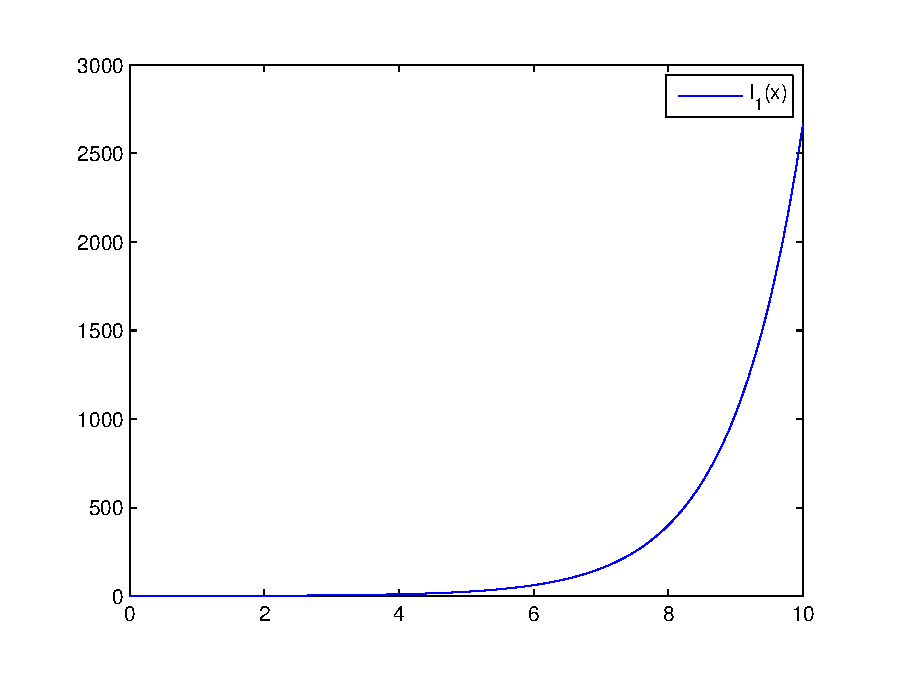
\includegraphics[width=.40\textwidth]{Bessel/BesselI.eps}&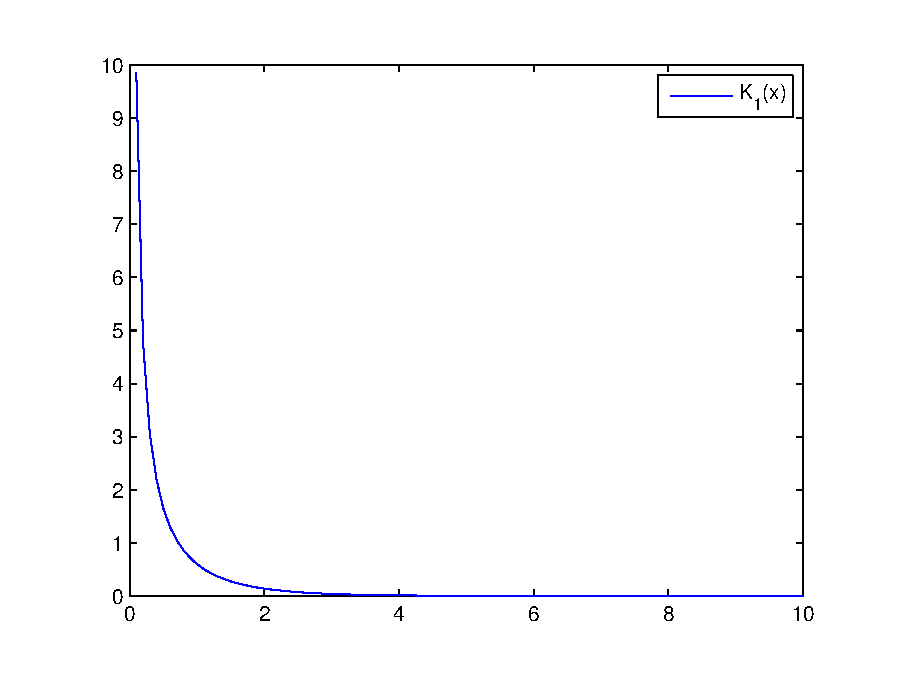
\includegraphics[width=.40\textwidth]{Bessel/BesselK.eps}\\\hline
		$J_\alpha(t)$&$Y_\alpha(t)$\\\hline
		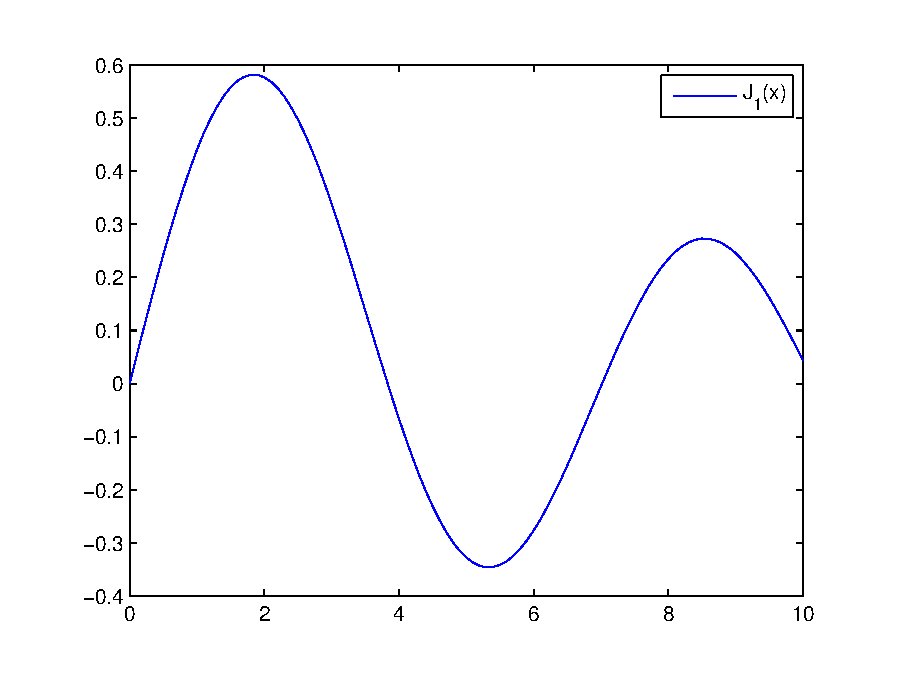
\includegraphics[width=.40\textwidth]{Bessel/BesselJ.eps}&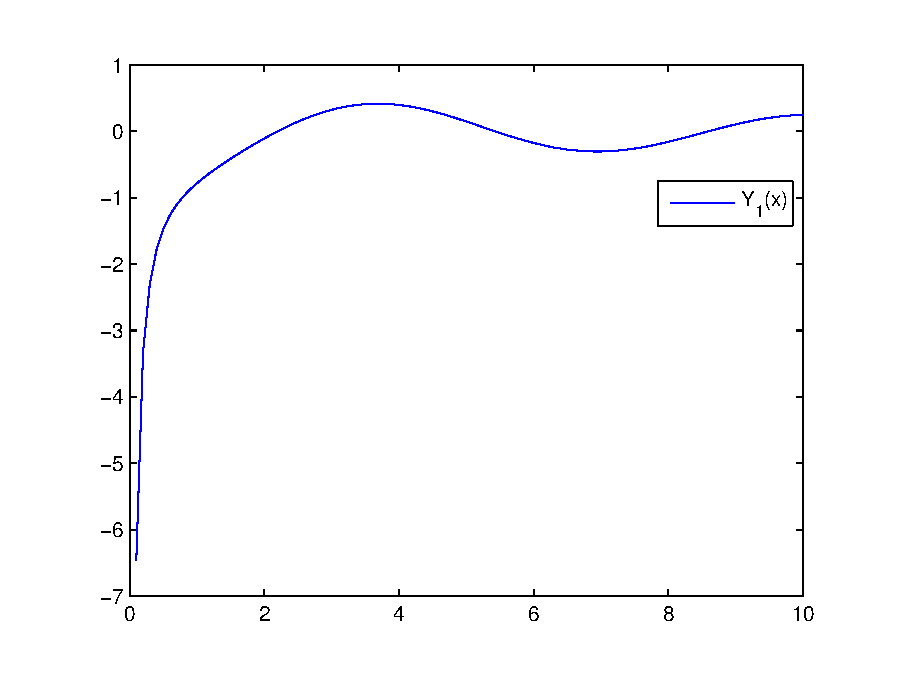
\includegraphics[width=.40\textwidth]{Bessel/BesselY.eps}\\\hline
		\end{tabular}\\
	\end{frame}
	
	
	
	
	
	
	
	
	
	\begin{frame}
		\frametitle{Solution Part 4}
		 We now conciser different values of $c$. We will only check the case where $c<0$ as the cases where $c=0$ and $c>0$ give trivial solutions.\\
		Letting $p=-c$, we can further 'simplify' $\varphi$ to 
		\[\varphi=D_1 i^\alpha J_\alpha(\sqrt{p}L)+D_2\left[\cot(\pi \alpha)-i^{-\alpha}Y_\alpha(L\sqrt{p})\right]\]
		Applying the first boundary condition we see that 
		\[0=D_1 i^\alpha J_\alpha(0)+D_2\left[\cot(\pi \alpha)-i^{-\alpha}Y_\alpha(0)\right]\]
		So $D_2=0$
	\end{frame}
	
	
	
		\begin{frame}
		\frametitle{Solution Part 5}
		 We now have $\varphi=D_1 i^\alpha J_\alpha(\sqrt{p}L)$. Using the second boundary condition gives
		\[
		D_1\left[-\alpha i^\alpha J_\alpha(L\sqrt{P})+Li^\alpha J'_\alpha(L\sqrt{p})\right]=0
		\]
		Simplifying we can write
		\begin{equation}
		J_{\alpha+1}(L\sqrt{p_n})=0\label{p}
		\end{equation}
		So our solutions for $\varphi$ are $\varphi=D_1i^\alpha J_\alpha(\sqrt{p_n}\sigma)$ where $p_n$ is a solution to \eqref{p}. Recalling that $\varphi=X(\sigma)\sigma ^\alpha$ we have
		\[
		X(\sigma)=\frac{J_\alpha(\sqrt{p_n}\sigma)}{\sigma^\alpha}
		\]
	\end{frame}
	
	
	
	\begin{frame}
		\frametitle{Solution Part 6}
		Recalling that our initial assumption was $\Phi(\sigma,\lambda)=T(\lambda)X(\sigma)$, we have
		\[
		\Phi(\sigma,\lambda)=\sum_{n=0}^\infty T_n(\lambda)\frac{J_\alpha(\sqrt{p_n}\sigma)}{\sigma^\alpha}
		\]
		We now solve the second ODE for $T$. Recall that
		$$T''(\lambda)=-p_nT(\lambda)$$
		The solution is:
		\[T(\lambda)=C_n \sin(\sqrt{p_n}\lambda)+D_n\cos(\sqrt{p_n}\lambda)\]
		So
		\[
		\Phi(\sigma,\lambda)=\sum_{n=0}^\infty C_n\frac{J_\alpha(\sqrt{p_n}\sigma)}{\sigma^\alpha} \sin(\sqrt{p_n}\lambda)+D_n\frac{J_\alpha(\sqrt{p_n}\sigma)}{\sigma^\alpha}\cos(\sqrt{p_n}\lambda)
		\]
	\end{frame}
	
	
	
	
		\begin{frame}
		\frametitle{Solution Part 7}
		Finally we use the ICs to write
		\[
		\sum_{n=0}^\infty D_n\frac{J_\alpha(\sqrt{p_n}\sigma)}{\sigma^\alpha}=\int\limits_0^\sigma u_0(\sigma ')F(\sigma ')d \sigma'
		\] and
		\[
		\sum_{n=0}^\infty C_n\sqrt{p_n}\frac{J_\alpha(\sqrt{p_n}\sigma)}{\sigma^\alpha} =2g\eta_0
		\]
		 Our final solution is:
				\[
		\Phi(\sigma,\lambda)=\sum_{n=0}^\infty C_n\frac{J_\alpha(\sqrt{p_n}\sigma)}{\sigma^\alpha} \sin(\sqrt{p_n}\lambda)+D_n\frac{J_\alpha(\sqrt{p_n}\sigma)}{\sigma^\alpha}\cos(\sqrt{p_n}\lambda)
		\]
		Where $J_{\alpha+1}(L\sqrt{p_n})=0$.
	\end{frame}
	
	
		\begin{frame}
		\frametitle{Numerical Implementation}
		To efficiently find the coefficients in the numerical code we solve the matrix systems
		\[
		\begin{pmatrix}
		\frac{J_\alpha(\sqrt{p_1}\sigma_1)}{\sigma_1^\alpha}&\ldots &\frac{J_\alpha(\sqrt{p_m}\sigma_1)}{\sigma_1^\alpha}\\
		\vdots&\ddots&\vdots\\
		\frac{J_\alpha(\sqrt{p_1}\sigma_n)}{\sigma_n^\alpha}&\ldots&\frac{J_\alpha(\sqrt{p_m}\sigma_n)}{\sigma_n^\alpha}\\
		\end{pmatrix}\begin{pmatrix}D_1\\\vdots\\D_m\end{pmatrix}=\begin{pmatrix} \int\limits_0^{\sigma_1} u_0(\sigma ')F(\sigma ')d \sigma'\\\vdots \\\int\limits_0^{\sigma_n} u_0(\sigma ')F(\sigma ')d \sigma' \end{pmatrix}
		\]
		and
				\[
		\begin{pmatrix}
		\frac{\sqrt{p_1}J_\alpha(\sqrt{p_1}\sigma_1)}{\sigma_1^\alpha}&\ldots &\frac{\sqrt{p_m}J_\alpha(\sqrt{p_m}\sigma_1)}{\sigma_1^\alpha}\\
		\vdots&\ddots&\vdots\\
		\frac{\sqrt{p_1}J_\alpha(\sqrt{p_1}\sigma_n)}{\sigma_n^\alpha}&\ldots&\frac{\sqrt{p_m}J_\alpha(\sqrt{p_m}\sigma_n)}{\sigma_n^\alpha}\\
		\end{pmatrix}\begin{pmatrix}C_1\\\vdots\\C_m\end{pmatrix}=\begin{pmatrix} 2g\eta_1\\\vdots \\2g\eta_n\end{pmatrix}
		\]
	\end{frame}
	
	
	
	
	
	
	
	
	
	
	
	
	
	
	
	
	
	
	
	
	
	
%	% 4  Results
% 4.1  Various plots with differing initial waves and bays ? including top-down view
% 4.1.1  Plots of same initial wave through different bays
% 4.1.1.1  Discuss resonance in terms of max. run up vs. max run up in plane-shaped bay (very large m)
% 4.1.1.1.1  Also in terms of how far up shore wave travels (top-down view)
% 4.1.2  Include at least one plot of eigenfunctions in both physical and sigma space
% 4.1.3  Include error in x wall mentioned previously in all different plots
% 4.2  Comparison to Pelinovsky?s analytic solution for m=2 and initial profile from paper
% 4.2.1  Comparison to initial condition
% 4.2.2  Alter number of eigenvalues, sigma (or x) steps, and lambda steps (each separately) to see what it takes to converge to analytic solution.
% 4.3  Possibly use max. run up and min. run down as a convergence metric - when varying number of eigenvalues, sigma (or x) steps, and lambda steps - for other values of m
% 4.4  Show how closely nonlinear system follows superposition principle ? measure of how linear/nonlinear the system is

\section{Results}

	\slide[RESULTS UNDER CONSTRUCTION]{}
%	% 5  Conclusion
% 5.1  Discuss strengths and weaknesses within model.
% 5.2  Future improvements/future work.
% 5.3  Acknowledgements
% 5.4  Bibliography

\section{Conclusion}
	\begin{frame}
		\frametitle{Future Problems}
		Our techniques can numerically solve any model such that:
		\be
			\item $u(x,t=0) = 0$.
			\item $f(y)$ is monotone non-increasing on $y \leq 0$ and non-decreasing on $y \geq 0$.
		\ee
	\end{frame}
	
	\begin{frame}
		\frametitle{Future Problems: Non-zero initial $u$}
		What if $u(x,t=0) \neq 0$?\\
		Matt postulated that our technique would work if $u(x,t=0)$ has a similar shape to $\eta(x,t=0)$.
	\end{frame}

	\begin{frame}
		\frametitle{Future Problems: W-bumps}
		What if we have W-bumps?
		\begin{center}
			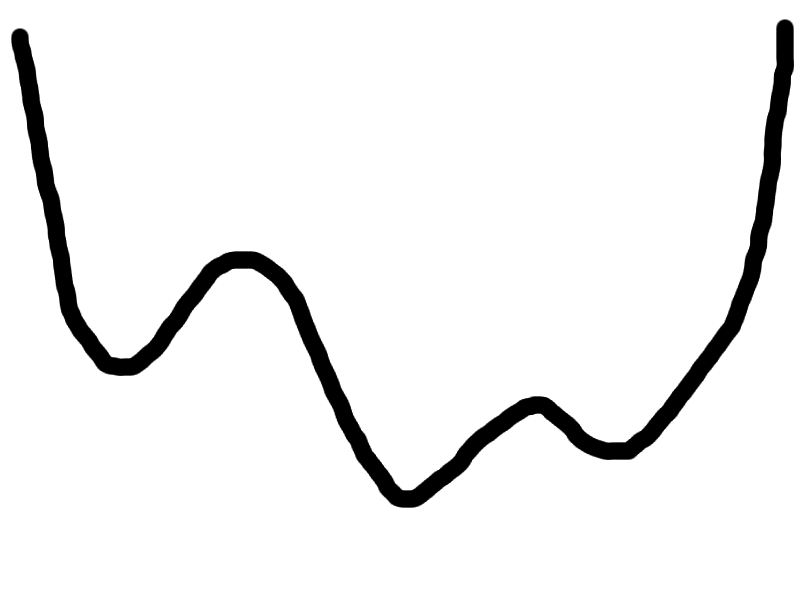
\includegraphics[width = 0.4\textwidth]{wbumps1.png}
			\quad
			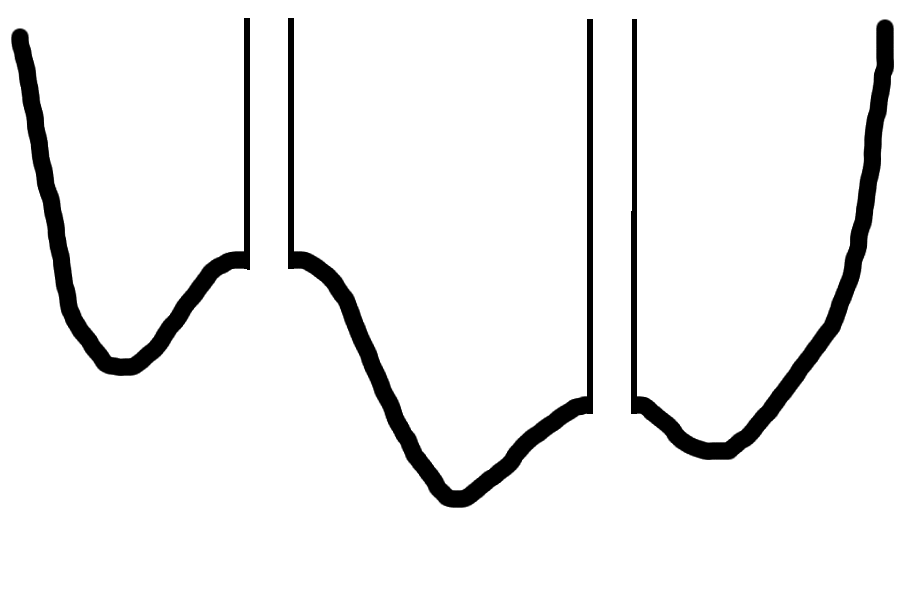
\includegraphics[width = 0.45\textwidth]{wbumps2.png}
		\end{center}
		Can we split into separate bays and analyse them separately?\\
		There are problems.
	\end{frame}


	\begin{frame}
		\frametitle{Acknowledgments}
	
		\begin{itemize}
		\item Dr. Alexei Rybkin  
		\item Dr. Dmitry Nicolsky
		\item Dr. Efim Pelinovsky
		\item Viacheslav Garayshin
		\item National Science Foundation
		\item University of Alaska Fairbanks
		\end{itemize}
		\end{frame}
	
		\begin{frame}[allowframebreaks]
		\nocite{*}
		\frametitle{Bibliography}
		\bibliographystyle{alpha}
		\bibliography{bibliography}
	\end{frame}
\end{document}
